\documentclass[11pt]{article}
\usepackage[margin=1in]{geometry}
\usepackage{amsmath,amssymb,amsthm,mathtools}
\usepackage{graphicx,booktabs,enumitem,array}
\usepackage[dvipsnames]{xcolor}
\usepackage{listings}
\usepackage[most]{tcolorbox}
\usepackage[hidelinks]{hyperref}
\setlength{\parindent}{0pt}
\setlength{\parskip}{0.55em}

% ---------- code styles ----------
\lstdefinestyle{py}{language=Python,basicstyle=\ttfamily\small,
  keywordstyle=\color{RoyalBlue}\bfseries,commentstyle=\color{OliveGreen},
  stringstyle=\color{BrickRed},backgroundcolor=\color{gray!6},frame=single,
  rulecolor=\color{gray!40},showstringspaces=false,columns=fullflexible,
  keepspaces=true,breaklines=true}
\lstdefinestyle{pynum}{style=py,numbers=left,numberstyle=\tiny\color{gray}}
\lstdefinestyle{out}{basicstyle=\ttfamily\small,backgroundcolor=\color{yellow!8},
  frame=leftline,rulecolor=\color{orange!70},columns=fullflexible,keepspaces=true}

% ---------- boxes ----------
\newtcolorbox{defbox}[1]{colback=blue!3,colframe=blue!45!black,fonttitle=\bfseries,title={#1},breakable}
\newtcolorbox{keybox}[1]{colback=green!3,colframe=green!40!black,fonttitle=\bfseries,title={#1},breakable}
\newtcolorbox{warnbox}[1]{colback=orange!4,colframe=orange!70!black,fonttitle=\bfseries,title={#1},breakable}

\newtheorem{proposition}{Proposition}
\newtheorem{lemma}{Lemma}
\theoremstyle{remark}\newtheorem{remark}{Remark}

\newcommand{\R}{\mathbb{R}}
\newcommand{\xh}{\hat{x}}
\newcommand{\Ah}{\hat{A}}
\newcommand{\At}{\tilde{A}}

\title{Reduced-Order Models and Operator Inference\\[2pt]
\large A self-contained note with one toy example worked by hand and in code}
\author{Lazizbek Sadullaev\\ \small Department of Mathematics and Statistics, Washington State University}
\date{November 2026}

\begin{document}
\maketitle

\begin{abstract}
This note explains, from scratch, what a projection-based reduced-order model (ROM) is, how the POD basis is obtained from the SVD, what ``intrusive'' and ``non-intrusive'' mean, and what Operator Inference (OpInf) of Peherstorfer and Willcox~\cite{PW16} does. Everything is illustrated on a single toy problem: the heat equation on 7 grid points, reduced to 2 dimensions. For this problem every number can be computed by hand; we do so step by step and check each number against Python. A second, slightly modified example shows when OpInf and the intrusive ROM differ, and how the re-projection idea of~\cite{P20} removes the difference. The note can be read on its own; the code in the folder \texttt{code/} reproduces all numbers and figures.
\end{abstract}

\tableofcontents

%=====================================================================
\section{How to read this note}
\begin{itemize}[leftmargin=1.5em]
\item Sections~\ref{sec:why}--\ref{sec:opinf} give the background: definitions, the main formulas and why they hold. Each key definition is in a blue box.
\item Section~\ref{sec:toy} sets up the toy problem, Section~\ref{sec:hand} solves it by hand (8 steps), and Section~\ref{sec:code} walks through the code block by block. Section~\ref{sec:mini} shows each numpy function on a tiny array with its literal output.
\item Section~\ref{sec:ex2} is a second experiment (closure error and re-projection). Section~\ref{sec:takeaways} lists the take-aways and where this connects to sparse regression (SINDy, MCP penalties).
\end{itemize}
Files in \texttt{code/} (only \texttt{numpy} and \texttt{matplotlib} are needed):
\begin{itemize}[leftmargin=1.5em,itemsep=0pt]
\item \texttt{opinf\_heat\_demo.py}: the main script (Section~\ref{sec:code});
\item \texttt{hand\_check.py}: checks every number of the hand calculation (Section~\ref{sec:hand});
\item \texttt{closure\_reprojection.py}: Example~2 (Section~\ref{sec:ex2});
\item \texttt{make\_figures.py}, \texttt{mini\_examples.py}: the figures and Section~\ref{sec:mini}.
\end{itemize}

%=====================================================================
\section{Why reduced-order models?}\label{sec:why}
Discretizing a PDE in space gives a system of ODEs (or, after time stepping, a recursion) for a state vector $x\in\R^N$ with $N$ often $10^4$--$10^7$. This is the \emph{full-order model} (FOM). Solving it once may be fine; solving it thousands of times (design, optimization, uncertainty quantification, control, a digital twin that must update in real time) is not.

The observation behind ROMs is that the states actually visited by the FOM usually lie close to a \emph{low-dimensional} subspace (or manifold). If we can find a basis $V\in\R^{N\times r}$ of that subspace with $r\ll N$, we can write $x\approx V\xh$ and evolve only the $r$ numbers $\xh$. Three questions then arise:
\begin{enumerate}[leftmargin=1.5em]
\item \textbf{Which basis?} Answer here: POD, computed from the SVD of snapshots (Section~\ref{sec:pod}).
\item \textbf{Which equation for $\xh$?} Classical answer: Galerkin projection of the FOM equations (Section~\ref{sec:galerkin}). This needs the FOM operators.
\item \textbf{What if we cannot access the FOM operators?} Answer: learn the reduced operators from data, which is Operator Inference (Section~\ref{sec:opinf}).
\end{enumerate}

%=====================================================================
\section{Projection-based ROMs}\label{sec:rom}
\subsection{The full-order model}
To keep things simple we use a linear, discrete-time FOM,
\begin{equation}\label{eq:fom}
x_{k+1}=A\,x_k,\qquad k=0,1,\dots,K-1,\qquad x_k\in\R^N,
\end{equation}
which is what one gets from a linear PDE after spatial discretization and an explicit Euler time step. The general case treated in~\cite{PW16,KPW24} is a continuous-time polynomial system
\begin{equation}\label{eq:poly}
\dot x = c + A x + H\,(x\otimes x) + B u ,
\end{equation}
with a constant term $c$, linear operator $A$, quadratic operator $H$ and input $u$. Everything below carries over; Section~\ref{sec:general} shows how.

\subsection{Basis, projection and lifting}
Let $V=[v_1,\dots,v_r]\in\R^{N\times r}$ have orthonormal columns, $V^\top V=I_r$.
\begin{itemize}[leftmargin=1.5em]
\item \textbf{Projection (encode):} $\xh=V^\top x\in\R^r$, the coordinates of $x$ in the basis.
\item \textbf{Lifting (decode):} $V\xh\in\R^N$.
\item $P=VV^\top$ is the orthogonal projector onto $\mathrm{range}(V)$: $P^2=P$, $P^\top=P$, and $Px$ is the closest point of $\mathrm{range}(V)$ to $x$. The error $x-Px$ is the part of $x$ the ROM cannot see.
\end{itemize}

\subsection{Galerkin projection: the intrusive ROM}\label{sec:galerkin}
Insert $x_k\approx V\xh_k$ into~\eqref{eq:fom}. The residual $V\xh_{k+1}-AV\xh_k$ cannot be zero in general (it lives in $\R^N$, we have only $r$ unknowns). Galerkin projection asks that it be \emph{orthogonal to the basis}: $V^\top(V\xh_{k+1}-AV\xh_k)=0$. Using $V^\top V=I$:
\begin{equation}\label{eq:galerkin}
\xh_{k+1}=\At\,\xh_k,\qquad \At = V^\top A V\in\R^{r\times r}.
\end{equation}
For~\eqref{eq:poly} the same recipe gives $\tilde c=V^\top c$, $\At=V^\top AV$, $\tilde H=V^\top H(V\otimes V)$, $\tilde B=V^\top B$.

\begin{defbox}{Definition (intrusive ROM)}
A ROM is \emph{intrusive} if building its operators requires the FOM operators, either as assembled matrices ($A$, $H$, \dots) or as a routine that returns products like $Av$. The Galerkin ROM~\eqref{eq:galerkin} is intrusive: we need $A$ to form $V^\top AV$.
\end{defbox}

\subsection{The POD basis}\label{sec:pod}
Collect snapshots as columns, $X=[x_0,x_1,\dots,x_K]\in\R^{N\times(K+1)}$.

\begin{defbox}{Definition (POD basis)}
The rank-$r$ POD basis is the $V$ with orthonormal columns that minimizes the total projection error of the snapshots,
\[
\min_{V^\top V=I_r}\ \sum_{k=0}^{K}\|x_k-VV^\top x_k\|_2^2 .
\]
\end{defbox}

\begin{keybox}{How to compute it: the SVD}
Write $X=U\Sigma W^\top$ (thin SVD) with singular values $\sigma_1\ge\sigma_2\ge\dots\ge0$. Then the POD basis is the first $r$ left singular vectors, $V=U_{:,1:r}$, and the minimal error equals $\sum_{j>r}\sigma_j^2$ (Eckart--Young theorem). Equivalently, $V$ consists of the leading eigenvectors of $XX^\top$, and $\sigma_j^2$ are its eigenvalues. The ratio $\sum_{j\le r}\sigma_j^2/\sum_j\sigma_j^2$ is the ``energy'' captured by $r$ modes and is the usual rule for choosing $r$.
\end{keybox}

In particular, \textbf{if $\mathrm{rank}(X)=r$, the snapshots lie exactly in $\mathrm{range}(V)$} and $x_k=VV^\top x_k$ for all $k$. This is the situation of our first toy example.

%=====================================================================
\section{Intrusive versus non-intrusive}\label{sec:intr}
In practice the FOM is often a large legacy or commercial code. It can be \emph{run} (give it an initial condition and inputs, it returns the trajectory), but its matrices are not available, or extracting them is impractical. Peherstorfer and Willcox call such a model a \emph{black box}~\cite[Sec.~1]{PW16}.

\begin{defbox}{Definition (non-intrusive ROM)}
A ROM is \emph{non-intrusive} if its operators are built only from data the FOM produces (initial conditions, inputs, state trajectories, outputs), without the FOM operators.
\end{defbox}

\begin{center}
\begin{tabular}{@{}lll@{}}
\toprule
& Intrusive (Galerkin) & Non-intrusive (OpInf) \\
\midrule
Needs & $A$ (or $v\mapsto Av$), basis $V$ & snapshots $X$, basis $V$ \\
Reduced operator & $\At=V^\top AV$ (formula) & $\Ah$ = least-squares fit \\
Structure of the ROM & polynomial, from the PDE & the same polynomial form, imposed \\
Guarantees & inherits properties of $A$ & equals $\At$ under conditions (Sec.~\ref{sec:equal}) \\
\bottomrule
\end{tabular}
\end{center}

A key point: OpInf does \emph{not} learn a black-box model. It keeps the \emph{form} of the projected equations (constant, linear, quadratic terms dictated by the PDE) and only learns the numbers in the reduced matrices. Willcox's group calls this learning a ``physics-based'' or ``structured'' reduced model~\cite{KPW24}.

%=====================================================================
\section{Operator Inference}\label{sec:opinf}
\subsection{Definition, discrete-time linear case}
Given snapshots $x_0,\dots,x_K$ and the POD basis $V$:
\begin{enumerate}[leftmargin=1.5em]
\item Project the data: $\xh_k=V^\top x_k$, $k=0,\dots,K$.
\item Choose the model form: here $\xh_{k+1}=\Ah\,\xh_k$.
\item Fit $\Ah$ by least squares:
\begin{equation}\label{eq:opinf}
\Ah=\arg\min_{M\in\R^{r\times r}}\ \sum_{k=0}^{K-1}\|\xh_{k+1}-M\xh_k\|_2^2 .
\end{equation}
\end{enumerate}

\begin{defbox}{Definition (Operator Inference)}
Operator Inference~\cite{PW16} infers the reduced operators of a projection-based ROM of prescribed (polynomial) form by solving a linear least-squares problem on the projected snapshot data, without using the FOM operators.
\end{defbox}

\paragraph{Matrix form.} Stack the data as rows:
\[
D=\begin{bmatrix}\xh_0^\top\\ \vdots\\ \xh_{K-1}^\top\end{bmatrix}\in\R^{K\times r},\qquad
R=\begin{bmatrix}\xh_1^\top\\ \vdots\\ \xh_{K}^\top\end{bmatrix}\in\R^{K\times r}.
\]
Transposing $\xh_{k+1}=\Ah\xh_k$ gives $\xh_{k+1}^\top=\xh_k^\top\Ah^\top$, i.e.\ $R\approx D\Ah^\top$. Hence~\eqref{eq:opinf} is
\begin{equation}\label{eq:lsq}
\min_{O}\ \|D\,O-R\|_F^2,\qquad O=\Ah^\top .
\end{equation}
If $D$ has full column rank $r$, the unique solution is $O=(D^\top D)^{-1}D^\top R$ (normal equations).

\paragraph{It splits into $r$ small problems.} The squared Frobenius norm is the sum over columns, so column $i$ of $O$ (= row $i$ of $\Ah$) solves its own problem $\min\|Do_i-r_i\|_2$, where $r_i$ is the time series of reduced coordinate $i$~\cite[eq.~(20)]{PW16}. This is exactly like SINDy, where each state equation is fitted separately.

\subsection{The general form}\label{sec:general}
For~\eqref{eq:poly} in continuous time, OpInf fits
\[
\frac{d\xh}{dt}=\hat c+\Ah\xh+\hat H(\xh\otimes\xh)+\hat Bu,
\]
with $D=[\,\mathbf 1,\ \hat X,\ \hat X^{(2)},\ U\,]$ (one row per time step: $1$, $\xh_k^\top$, the products $\xh_{k,i}\xh_{k,j}$ with $i\le j$, $u_k^\top$) and $R$ containing estimates of $d\xh/dt$ (e.g.\ finite differences)~\cite[Sec.~3.2]{PW16}. With noisy or poorly conditioned data one adds a Tikhonov (ridge) term,
\[
\min_O\ \|DO-R\|_F^2+\lambda\|O\|_F^2 ,
\]
see~\cite{KPW24}. In discrete time no derivative estimate is needed: $R$ is just the shifted data, as in~\eqref{eq:lsq}.

\subsection{When is OpInf equal to the intrusive ROM?}\label{sec:equal}
\begin{proposition}[Exact recovery when the data lie in the subspace]\label{prop:exact}
Suppose $x_k=VV^\top x_k$ for $k=0,\dots,K-1$ (the snapshots lie in $\mathrm{range}(V)$) and $D$ has full column rank. Then $\Ah=\At=V^\top AV$.
\end{proposition}
\begin{proof}
$\xh_{k+1}=V^\top x_{k+1}=V^\top Ax_k=V^\top A(VV^\top x_k)=(V^\top AV)\,\xh_k$. So $R=D\At^\top$ exactly, the objective of~\eqref{eq:lsq} is zero at $O=\At^\top$, and by full column rank this minimizer is unique.
\end{proof}

\begin{warnbox}{In general the data are \emph{not} in the subspace: closure error}
Write $x_k=V\xh_k+e_k$ with $e_k\perp\mathrm{range}(V)$. Then
\[
\xh_{k+1}=\At\xh_k+\underbrace{V^\top A e_k}_{\text{closure term}} .
\]
The projected data contain the effect of the truncated modes, which a model $\xh_{k+1}=M\xh_k$ cannot represent. Least squares then returns some $\Ah\neq\At$. Peherstorfer and Willcox show $\Ah\to\At$ as the time step goes to $0$ and $r\to N$~\cite[Thm.~1]{PW16}; Peherstorfer~\cite{P20} shows exact recovery for finite data with a modified sampling, \emph{re-projection}: instead of taking FOM trajectories, start from the lifted reduced state $V\xh_k$, take one FOM step and project again,
\[
\bar x_{k+1}=V^\top\,\mathrm{FOM\_step}(V\bar x_k).
\]
For~\eqref{eq:fom} this gives $\bar x_{k+1}=V^\top AV\bar x_k=\At\bar x_k$, so the data are Markovian in the reduced space and Proposition~\ref{prop:exact} applies. Section~\ref{sec:ex2} shows this numerically.
\end{warnbox}

\subsection{Relation to DMD and SINDy}
\begin{center}
\begin{tabular}{@{}>{\raggedright}p{1.6cm}>{\raggedright}p{4.2cm}>{\raggedright}p{4.6cm}>{\raggedright\arraybackslash}p{3.4cm}@{}}
\toprule
& Model form & Regression & Coordinates \\
\midrule
DMD & linear, $x_{k+1}\approx Mx_k$ & least squares & full or POD \\
OpInf & polynomial, fixed by the PDE & least squares (+ Tikhonov) & POD \\
SINDy & large library of candidates & sparse regression (STLSQ, LASSO, MCP, \dots) & any (often measured) \\
\bottomrule
\end{tabular}
\end{center}
For a linear FOM without time-varying inputs, the OpInf operator coincides with the DMD operator~\cite[Sec.~1]{PW16}. OpInf and SINDy solve the same kind of regression; they differ in how the library is chosen (physics vs.\ data) and in the penalty.

%=====================================================================
\section{The toy problem}\label{sec:toy}
Heat equation on $[0,1]$ with zero boundary values,
\[
u_t=u_{\xi\xi},\qquad u(0,t)=u(1,t)=0 .
\]
Grid: $\xi_i=i\,\Delta\xi$, $\Delta\xi=1/8$, interior points $i=1,\dots,7$, so $N=7$. Central differences give $\dot x=Lx$ with the tridiagonal matrix
\[
L=\frac{1}{\Delta\xi^2}\begin{bmatrix}-2&1&&&\\1&-2&1&&\\&\ddots&\ddots&\ddots&\\&&1&-2&1\\&&&1&-2\end{bmatrix}\in\R^{7\times7}.
\]
Explicit Euler with $\Delta t=0.004$ gives the FOM~\eqref{eq:fom} with $A=I+\Delta t\,L$. Initial condition and data:
\[
x_0(i)=\sin(\pi i/8)+\tfrac12\sin(3\pi i/8),\qquad K=40\ \text{steps},\qquad r=2 .
\]

\begin{figure}[h]\centering
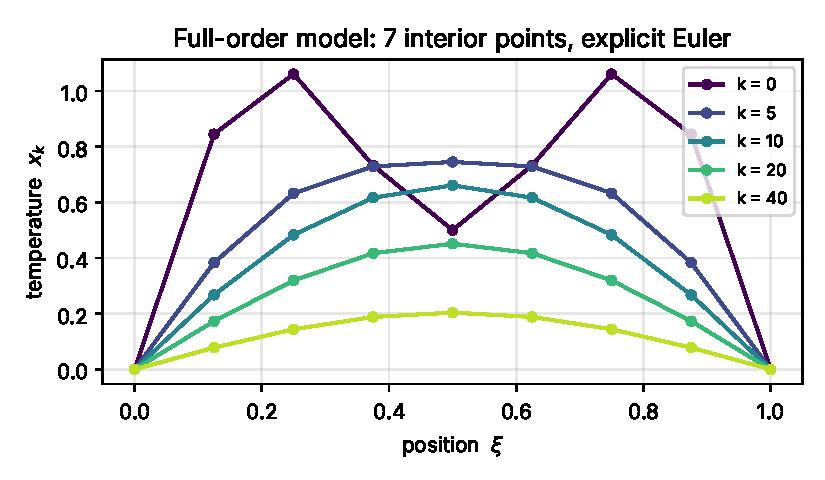
\includegraphics[width=0.72\textwidth]{figures/fig1_snapshots.pdf}
\caption{FOM snapshots (boundary zeros added). The bumpy part (mode $j=3$) dies out faster than the smooth part ($j=1$).}\label{fig:snap}
\end{figure}

%=====================================================================
\section{The example by hand}\label{sec:hand}
All numbers below are reproduced by \texttt{code/hand\_check.py}; its output is printed at the end of this section.

\subsection*{Step 1. The key number}
$\Delta t/\Delta\xi^2=0.004\times64=0.256$. (Explicit Euler for the heat equation is stable if this is $\le 1/2$.)

\subsection*{Step 2. Eigenvectors and eigenvalues of $A$}
Let $v_j(i)=\sin(j\pi i/8)$, $j=1,\dots,7$. With $a=j\pi i/8$, $b=j\pi/8$ and $\sin(a-b)+\sin(a+b)=2\sin a\cos b$,
\[
(Lv_j)_i=\frac{\sin(a-b)-2\sin a+\sin(a+b)}{\Delta\xi^2}=\frac{2\cos b-2}{\Delta\xi^2}\sin a
=-\frac{4\sin^2(j\pi/16)}{\Delta\xi^2}\,v_j(i),
\]
using $1-\cos b=2\sin^2(b/2)$. At the ends the formula needs $v_j(0)=\sin0=0$ and $v_j(8)=\sin(j\pi)=0$, which is exactly the zero boundary condition, so the formula holds for every row of $L$. Hence $Av_j=a_jv_j$ with
\[
\boxed{a_j=1-4\,\tfrac{\Delta t}{\Delta\xi^2}\sin^2\!\tfrac{j\pi}{16}=1-1.024\,\sin^2\!\tfrac{j\pi}{16}}
\]
\[
a_1=1-1.024\,(0.19509)^2=0.961026,\qquad a_3=1-1.024\,(0.55557)^2=0.683934 .
\]
Interpretation: per time step the smooth mode keeps $96.1\%$ of its amplitude, the bumpy mode only $68.4\%$.

\subsection*{Step 3. Normalizing}
$\|v_j\|^2=\sum_{i=1}^7\sin^2(j\pi i/8)=\tfrac72-\tfrac12\sum_{i=1}^7\cos(j\pi i/4)=\tfrac72+\tfrac12=4$, because $\sum_{i=0}^{7}\cos(j\pi i/4)=0$ for $j=1,\dots,7$ (a full sum of 8th roots of unity), so the sum from $i=1$ is $-1$. The $v_j$ are orthogonal (eigenvectors of the symmetric matrix $L$ with distinct eigenvalues). So
\[
q_j=v_j/2\quad\text{are orthonormal.}
\]

\subsection*{Step 4. The trajectory in closed form}
$x_0=v_1+\tfrac12v_3=2q_1+q_3$, and $A$ multiplies each eigenvector by its eigenvalue, so
\[
\boxed{x_k=A^kx_0=2a_1^k\,q_1+a_3^k\,q_3 .}
\]
Every snapshot lies in the plane $\mathrm{span}\{q_1,q_3\}$, hence $\mathrm{rank}(X)=2$.

\subsection*{Step 5. The singular values}
Write $X=Q\,C$ with $Q=[q_1\ q_3]\in\R^{7\times2}$ ($Q^\top Q=I$) and
\[
C=\begin{bmatrix}2a_1^0&2a_1^1&\cdots&2a_1^{40}\\ a_3^0&a_3^1&\cdots&a_3^{40}\end{bmatrix}\in\R^{2\times41}.
\]
Then $XX^\top=Q\,G\,Q^\top$ with $G=CC^\top$. If $Gw=\lambda w$ then $XX^\top(Qw)=\lambda\,Qw$, so the nonzero eigenvalues of $XX^\top$ are those of $G$: $\sigma_j=\sqrt{\lambda_j(G)}$, and the left singular vectors are $Qw$. The entries of $G$ are geometric sums, $\sum_{k=0}^{40}\rho^k=(1-\rho^{41})/(1-\rho)$:
\[
G_{11}=4\sum a_1^{2k}=4\frac{1-a_1^{82}}{1-a_1^2}=50.327,\quad
G_{33}=\frac{1-a_3^{82}}{1-a_3^2}=1.8789,\quad
G_{13}=2\frac{1-(a_1a_3)^{41}}{1-a_1a_3}=5.8356 .
\]
For a symmetric $2\times2$ matrix, $\lambda=m\pm d$ with $m=\tfrac{G_{11}+G_{33}}2=26.103$ and $d=\sqrt{(\tfrac{G_{11}-G_{33}}2)^2+G_{13}^2}=24.917$:
\[
\lambda_1=51.020,\ \lambda_2=1.1859\quad\Longrightarrow\quad\boxed{\sigma_1=7.1428,\ \sigma_2=1.0890,\ \sigma_3=\dots=\sigma_7=0.}
\]
With $r=2$ the POD captures $100\%$ of the energy.

\subsection*{Step 6. The POD basis is a rotated $\{q_1,q_3\}$}
The unit eigenvector of $G$ for $\lambda_1$ is $w_1=(\cos\theta,\sin\theta)$ with
\[
\tan2\theta=\frac{2G_{13}}{G_{11}-G_{33}}=\frac{11.671}{48.448}=0.2409,\qquad \theta=0.1182\text{ rad}=6.77^\circ,
\]
and $w_2=(-\sin\theta,\cos\theta)$. Thus $V=QW$ with the rotation $W=[w_1\ w_2]$:
\[
v^{\rm POD}_1=\cos\theta\,q_1+\sin\theta\,q_3,\qquad v^{\rm POD}_2=-\sin\theta\,q_1+\cos\theta\,q_3 ,
\]
with $\cos\theta=0.9930$, $\sin\theta=0.1179$ (Figure~\ref{fig:modes}). A numerical SVD may flip the sign of any column; this changes only the sign of the off-diagonal entry below.

\begin{figure}[h]\centering
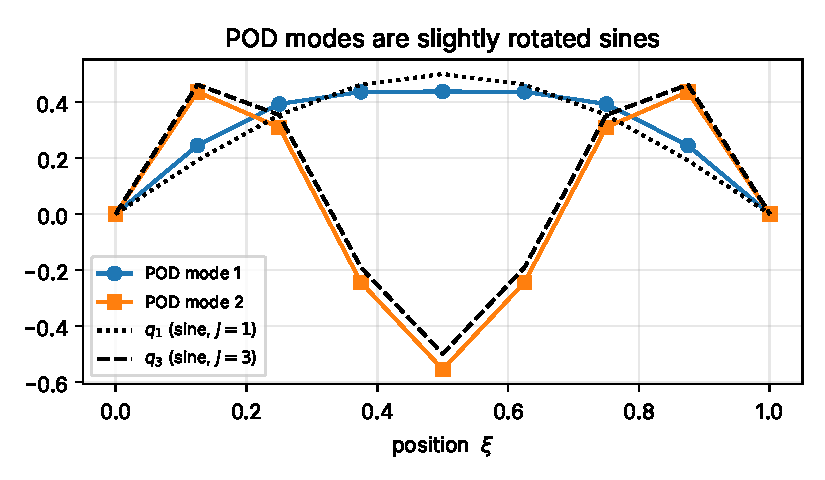
\includegraphics[width=0.72\textwidth]{figures/fig3_pod_modes.pdf}
\caption{POD modes compared with $q_1$, $q_3$: the first POD mode is mostly $q_1$ with a little $q_3$ mixed in ($\theta\approx6.8^\circ$).}\label{fig:modes}
\end{figure}

\subsection*{Step 7. The intrusive reduced operator}
$\At=V^\top AV=W^\top(Q^\top AQ)W=W^\top\mathrm{diag}(a_1,a_3)\,W$, because $AQ=Q\,\mathrm{diag}(a_1,a_3)$. Multiplying out:
\[
\At_{11}=a_1\cos^2\theta+a_3\sin^2\theta=0.9572,\qquad
\At_{22}=a_1\sin^2\theta+a_3\cos^2\theta=0.6878,
\]
\[
\At_{12}=\At_{21}=-(a_1-a_3)\cos\theta\sin\theta=-0.0324 .
\]
Checks: $\mathrm{tr}\,\At=1.6450=a_1+a_3$ and $\det\At=0.6573=a_1a_3$. So $\At$ is just $\mathrm{diag}(0.961,0.684)$ seen in slightly rotated coordinates; its eigenvalues are exactly the two decay factors.

\subsection*{Step 8. Operator Inference gives the same matrix}
By Step~4 the snapshots lie in $\mathrm{range}(V)$, and $D$ has rank $2$ (the reduced states are not all parallel, since the two modes decay at different rates). Proposition~\ref{prop:exact} gives
\[
\boxed{\Ah=\At=\begin{bmatrix}0.9572&-0.0324\\-0.0324&0.6878\end{bmatrix}}
\]
without ever using $A$: OpInf only saw the 41 snapshots.

\paragraph{Output of \texttt{hand\_check.py}.}
\lstinputlisting[style=out]{generated/hand_check.out}

\begin{center}
\begin{tabular}{@{}lll@{}}
\toprule
Quantity & by hand & code \\
\midrule
$a_1,\ a_3$ & $0.9610,\ 0.6839$ & \texttt{0.961026, 0.683934} \\
$\sigma_1,\ \sigma_2$ & $7.1428,\ 1.0890$ & \texttt{7.1428, 1.089} \\
$\theta$ & $6.77^\circ$ & \texttt{6.772 deg} \\
$\At_{11},\ \At_{22},\ \At_{12}$ & $0.9572,\ 0.6878,\ -0.0324$ & same \\
$\|\Ah-\At\|_F$ & $0$ & \texttt{4.9e-16} \\
\bottomrule
\end{tabular}
\end{center}

%=====================================================================
\section{The code, block by block}\label{sec:code}
The full script is in Appendix~\ref{app:code}. Here each block is shown with what it does and which step of Section~\ref{sec:hand} it corresponds to. Every numpy function is demonstrated on a tiny array in Section~\ref{sec:mini}.

\paragraph{Block 1: the FOM.}
\lstinputlisting[style=pynum,firstline=8,lastline=13,firstnumber=8]{../code/opinf_heat_demo.py}
Line 9 fixes $N=7$, $\Delta\xi=1/8$, $\Delta t=0.004$. Lines 10--12 build $L$: \texttt{np.diag(-2*np.ones(N))} puts $-2$ on the main diagonal, \texttt{np.diag(np.ones(N-1), 1)} puts $1$ just above it, \texttt{..., -1)} just below; the sum is divided by $\Delta\xi^2$. Line 13 is $A=I+\Delta t\,L$. (Hand: Step 1--2.)

\paragraph{Block 2: initial condition and snapshots.}
\lstinputlisting[style=pynum,firstline=15,lastline=23,firstnumber=15]{../code/opinf_heat_demo.py}
Line 16 creates the index vector $i=(1,\dots,7)$; line 17 evaluates $x_0(i)$ elementwise (numpy applies \texttt{np.sin} to every entry). Line 20 reserves a $7\times41$ matrix; line 21 stores $x_0$ in column $0$; the loop applies one FOM step per column, $x_{k+1}=Ax_k$. Only this ``run the model'' part touches $A$. (Hand: Step 4.)

\paragraph{Block 3: POD.}
\lstinputlisting[style=pynum,firstline=25,lastline=29,firstnumber=25]{../code/opinf_heat_demo.py}
\texttt{np.linalg.svd(X, full\_matrices=False)} returns $U$ ($7\times7$), the singular values \texttt{s} (largest first) and $W^\top$. Printing \texttt{s} shows two nonzero values, $7.1428$ and $1.089$ (Step 5). Line 29 keeps the first two columns: $V=U_{:,1:2}$ (Step 6).

\paragraph{Block 4: projection.}
\lstinputlisting[style=pynum,firstline=31,lastline=32,firstnumber=31]{../code/opinf_heat_demo.py}
One matrix product projects all 41 snapshots at once: column $k$ of \texttt{Xh} is $\xh_k=V^\top x_k\in\R^2$.

\paragraph{Block 5: Operator Inference.}
\lstinputlisting[style=pynum,firstline=34,lastline=38,firstnumber=34]{../code/opinf_heat_demo.py}
\texttt{Xh[:, :-1]} is $[\xh_0,\dots,\xh_{39}]$ and \texttt{Xh[:, 1:]} is $[\xh_1,\dots,\xh_{40}]$; the transposes stack them as rows, giving $D$ and $R$ of~\eqref{eq:lsq} ($40\times2$ each). \texttt{np.linalg.lstsq(D, R)} solves $\min\|DO-R\|_F$ for $O=\Ah^\top$, column by column; it also returns the residual, the rank of $D$ and its singular values. Line 38 transposes back to $\Ah$. (Step 8.)

\paragraph{Block 6: comparison with the intrusive ROM.}
\lstinputlisting[style=pynum,firstline=40,lastline=45,firstnumber=40]{../code/opinf_heat_demo.py}
Line 41 forms $V^\top AV$, which needs $A$; we compute it only to check. \texttt{np.linalg.norm} of the difference is the Frobenius norm, $\approx5\times10^{-16}$ (round-off). The eigenvalues of $\Ah$ are $a_1,a_3$ (Step 7).

\paragraph{Block 7: prediction.}
\lstinputlisting[style=pynum,firstline=47,lastline=53,firstnumber=47]{../code/opinf_heat_demo.py}
The ROM is run from $\xh_0=V^\top x_0$ for 40 steps of the $2\times2$ recursion, then lifted, $V\xh_{40}\in\R^7$, and compared with the FOM state.

\paragraph{Output of \texttt{opinf\_heat\_demo.py}.}
\lstinputlisting[style=out]{generated/opinf_heat_demo.out}

\begin{figure}[h]\centering
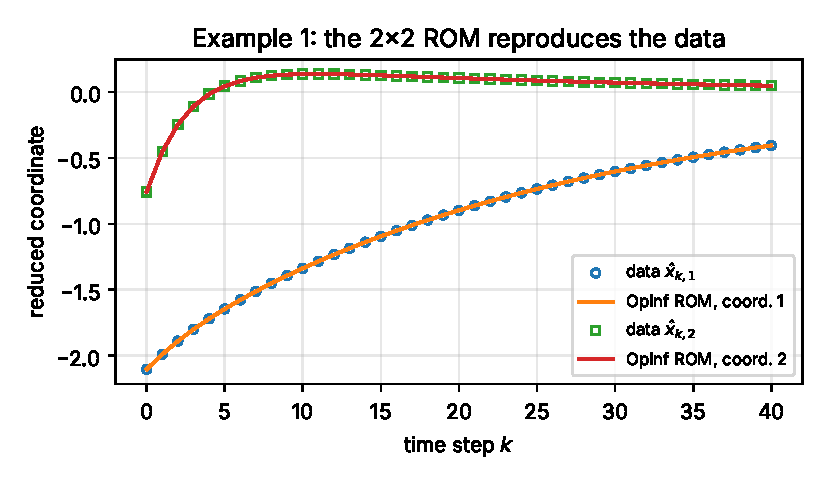
\includegraphics[width=0.72\textwidth]{figures/fig4_reduced_coords.pdf}
\caption{Reduced coordinates: projected data (markers) and the OpInf ROM run from $\xh_0$ (lines).}
\end{figure}

%=====================================================================
\section{Each numpy function on a tiny example}\label{sec:mini}
Generated by \texttt{code/mini\_examples.py}: the code is executed and its printed output is copied below unchanged.

\paragraph{\texttt{np.arange(start, stop)}} Integers from start up to stop-1. We use it for the grid index i = 1,...,7.

\begin{lstlisting}[style=py]
import numpy as np
i = np.arange(1, 8)
print(i)
print(i/8)
\end{lstlisting}

\begin{lstlisting}[style=out]
[1 2 3 4 5 6 7]
[0.125 0.25  0.375 0.5   0.625 0.75  0.875]
\end{lstlisting}

\paragraph{\texttt{np.ones(n) and np.zeros((m, n))}} Arrays filled with ones or zeros. zeros((m, n)) reserves space for the snapshot matrix.

\begin{lstlisting}[style=py]
import numpy as np
print(np.ones(5))
print(np.zeros((2, 5)))
\end{lstlisting}

\begin{lstlisting}[style=out]
[1. 1. 1. 1. 1.]
[[0. 0. 0. 0. 0.]
 [0. 0. 0. 0. 0.]]
\end{lstlisting}

\paragraph{\texttt{np.diag(v, k)}} Puts the vector v on the k-th diagonal of a square matrix (k = 0 main, k = 1 above, k = -1 below).

\begin{lstlisting}[style=py]
import numpy as np
print(np.diag([-2, -2, -2, -2, -2]))
print(np.diag([1, 1, 1, 1], 1))
\end{lstlisting}

\begin{lstlisting}[style=out]
[[-2  0  0  0  0]
 [ 0 -2  0  0  0]
 [ 0  0 -2  0  0]
 [ 0  0  0 -2  0]
 [ 0  0  0  0 -2]]
[[0 1 0 0 0]
 [0 0 1 0 0]
 [0 0 0 1 0]
 [0 0 0 0 1]
 [0 0 0 0 0]]
\end{lstlisting}

\paragraph{\texttt{Building the 1D Laplacian}} The sum of the three diagonals gives the tridiagonal matrix of Section 6 (here N = 5, without the 1/dx**2 factor).

\begin{lstlisting}[style=py]
import numpy as np
N = 5
T = np.diag(-2*np.ones(N)) + np.diag(np.ones(N-1), 1) + np.diag(np.ones(N-1), -1)
print(T)
\end{lstlisting}

\begin{lstlisting}[style=out]
[[-2.  1.  0.  0.  0.]
 [ 1. -2.  1.  0.  0.]
 [ 0.  1. -2.  1.  0.]
 [ 0.  0.  1. -2.  1.]
 [ 0.  0.  0.  1. -2.]]
\end{lstlisting}

\paragraph{\texttt{np.eye(n)}} The identity matrix. A = I + dt L is one explicit Euler step.

\begin{lstlisting}[style=py]
import numpy as np
print(np.eye(5))
\end{lstlisting}

\begin{lstlisting}[style=out]
[[1. 0. 0. 0. 0.]
 [0. 1. 0. 0. 0.]
 [0. 0. 1. 0. 0.]
 [0. 0. 0. 1. 0.]
 [0. 0. 0. 0. 1.]]
\end{lstlisting}

\paragraph{\texttt{The @ operator}} Matrix times vector (or matrix times matrix). One FOM step is A @ x.

\begin{lstlisting}[style=py]
import numpy as np
T = np.diag(-2*np.ones(5)) + np.diag(np.ones(4), 1) + np.diag(np.ones(4), -1)
x = np.array([0., 1., 2., 1., 0.])
print(T @ x)
\end{lstlisting}

\begin{lstlisting}[style=out]
[ 1.  0. -2.  0.  1.]
\end{lstlisting}

\paragraph{\texttt{Filling columns: X[:, k]}} X[:, k] is column k of X. The time loop writes the state x(k) into column k.

\begin{lstlisting}[style=py]
import numpy as np
X = np.zeros((3, 4))
X[:, 0] = [1., 2., 3.]
for k in range(3):
    X[:, k+1] = 0.5 * X[:, k]
print(X)
\end{lstlisting}

\begin{lstlisting}[style=out]
[[1.    0.5   0.25  0.125]
 [2.    1.    0.5   0.25 ]
 [3.    1.5   0.75  0.375]]
\end{lstlisting}

\paragraph{\texttt{Slicing: M[:, :-1] and M[:, 1:]}} All columns except the last, and all columns except the first. Side by side they pair x(k) with x(k+1).

\begin{lstlisting}[style=py]
import numpy as np
M = np.arange(10).reshape(2, 5)
print(M)
print(M[:, :-1])
print(M[:, 1:])
\end{lstlisting}

\begin{lstlisting}[style=out]
[[0 1 2 3 4]
 [5 6 7 8 9]]
[[0 1 2 3]
 [5 6 7 8]]
[[1 2 3 4]
 [6 7 8 9]]
\end{lstlisting}

\paragraph{\texttt{Transpose .T}} Swaps rows and columns. OpInf stacks the reduced states as ROWS of D, so we transpose.

\begin{lstlisting}[style=py]
import numpy as np
M = np.arange(6).reshape(2, 3)
print(M)
print(M.T)
\end{lstlisting}

\begin{lstlisting}[style=out]
[[0 1 2]
 [3 4 5]]
[[0 3]
 [1 4]
 [2 5]]
\end{lstlisting}

\paragraph{\texttt{np.linalg.svd(X, full\_matrices=False)}} X = U diag(s) Wt. Columns of U are the POD modes, s are the singular values (largest first). A rank-1 example: only one singular value is nonzero.

\begin{lstlisting}[style=py]
import numpy as np
np.set_printoptions(precision=4, suppress=True)
X = np.outer([1., 2., 2.], [1., 0.5, 0.25, 0.125, 0.0625])
U, s, Wt = np.linalg.svd(X, full_matrices=False)
print(s)
print(U[:, 0])
\end{lstlisting}

\begin{lstlisting}[style=out]
[3.4624 0.     0.    ]
[-0.3333 -0.6667 -0.6667]
\end{lstlisting}

\paragraph{\texttt{U[:, :r]}} The first r columns: the POD basis V.

\begin{lstlisting}[style=py]
import numpy as np
U = np.arange(15).reshape(5, 3)
print(U[:, :2])
\end{lstlisting}

\begin{lstlisting}[style=out]
[[ 0  1]
 [ 3  4]
 [ 6  7]
 [ 9 10]
 [12 13]]
\end{lstlisting}

\paragraph{\texttt{np.linalg.lstsq(D, R, rcond=None)}} Finds the M that makes the residual D M - R as small as possible (least squares). Here the data come from x(k+1) = 0.8 x(k) exactly, so the fitted slope is 0.8.

\begin{lstlisting}[style=py]
import numpy as np
x = 0.8**np.arange(6)            # 1, 0.8, 0.64, ...
D = x[:-1].reshape(-1, 1)        # column of x_k
R = x[1:].reshape(-1, 1)         # column of x_{k+1}
M, res, rank, sv = np.linalg.lstsq(D, R, rcond=None)
print(M)
\end{lstlisting}

\begin{lstlisting}[style=out]
[[0.8]]
\end{lstlisting}

\paragraph{\texttt{np.linalg.norm and np.linalg.eigvals}} The (Frobenius) norm measures the size of a difference; eigvals gives the eigenvalues of a matrix.

\begin{lstlisting}[style=py]
import numpy as np
np.set_printoptions(precision=4, suppress=True)
B = np.array([[0.9, 0.1], [0.1, 0.7]])
print(np.linalg.norm(B - np.diag([0.9, 0.7])))
print(np.linalg.eigvals(B))
\end{lstlisting}

\begin{lstlisting}[style=out]
0.14142135623730953
[0.9414+0.j 0.6586+0.j]
\end{lstlisting}


%=====================================================================
\section{Example 2: data outside the subspace}\label{sec:ex2}
Same FOM, but a third mode is added to the initial condition, while we keep $r=2$:
\[
x_0(i)=\sin(\pi i/8)+\tfrac12\sin(3\pi i/8)+0.4\,\sin(5\pi i/8).
\]
Now $\mathrm{rank}(X)=3$ (Figure~\ref{fig:sv}), so the snapshots do \emph{not} lie in the 2D POD space and Proposition~\ref{prop:exact} does not apply. The script \texttt{closure\_reprojection.py} computes three $2\times2$ operators: plain OpInf on FOM trajectories, OpInf on re-projected data (one black-box step from $V\bar x_k$, then projection), and the intrusive $V^\top AV$.

\begin{figure}[h]\centering
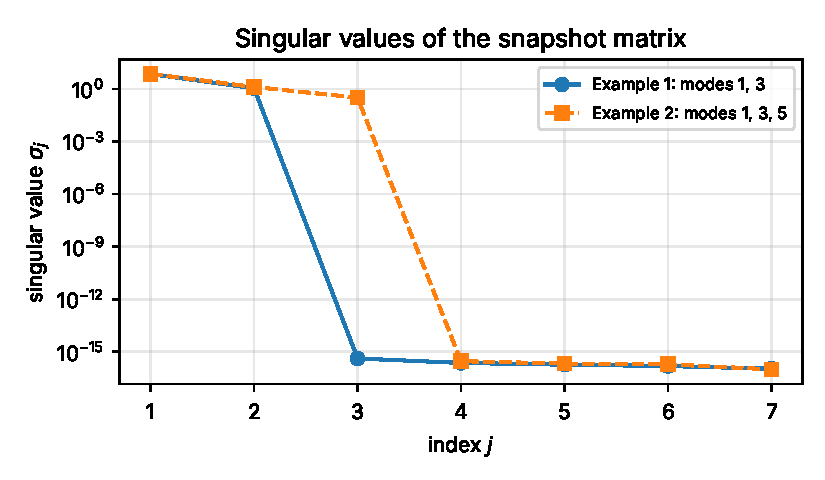
\includegraphics[width=0.72\textwidth]{figures/fig2_singular_values.pdf}
\caption{Singular values. Example~1 has exactly two nonzero values (the others are round-off and plotted at $10^{-17}$); Example~2 has three.}\label{fig:sv}
\end{figure}

\paragraph{Output of \texttt{closure\_reprojection.py}.}
\lstinputlisting[style=out]{generated/closure_reprojection.out}

\paragraph{What this shows.}
\begin{enumerate}[leftmargin=1.5em]
\item Plain OpInf is no longer exactly the intrusive ROM ($\|\Ah-\At\|_F\approx7\times10^{-5}$), because of the closure term $V^\top Ae_k$. With re-projection the difference drops to round-off, as predicted by~\cite{P20}.
\item Here the difference is tiny. The reason is that this FOM is very benign: $A$ is symmetric and the truncated part decays fast ($a_5\approx0.29$). For convection-dominated or nonlinear problems the closure effect can be large and plain OpInf can even be unstable while the re-projected one is not~\cite{P20}.
\item All three ROMs have the same maximal prediction error, about $8\%$ (Figure~\ref{fig:err}). This error is \emph{truncation}: a 2D model cannot represent the third mode at all. Two different errors should be kept apart: (i) the truncation error, set by $r$ and the basis, and (ii) the gap between learned and intrusive operators, set by the data.
\end{enumerate}

\begin{figure}[h]\centering
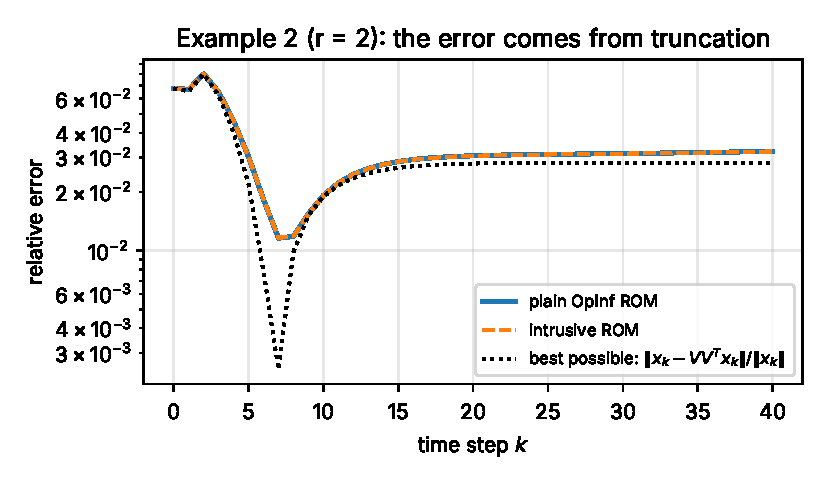
\includegraphics[width=0.72\textwidth]{figures/fig5_example2_errors.pdf}
\caption{Example 2: relative error of the plain OpInf ROM and the intrusive ROM, and the best possible error $\|x_k-VV^\top x_k\|/\|x_k\|$. The early peak is the truncated mode 5, which decays fastest. The error does not go to zero afterwards: the POD plane is fitted to all snapshots, so it does not contain $q_1$ exactly, and even the late states (almost pure mode 1) keep a relative error of about $3\%$.}\label{fig:err}
\end{figure}

%=====================================================================
\section{Take-aways and next steps}\label{sec:takeaways}
\begin{enumerate}[leftmargin=1.5em]
\item \textbf{ROM} $=$ basis $V$ (here POD from the SVD) $+$ an equation for the coordinates $\xh=V^\top x$.
\item \textbf{Intrusive (Galerkin)}: $\At=V^\top AV$, needs the FOM operators. \textbf{Non-intrusive (OpInf)}: $\Ah$ from least squares on projected snapshots, needs only data, but keeps the physics-dictated form.
\item If the data lie in the reduced space, OpInf recovers the intrusive ROM exactly (Proposition~\ref{prop:exact}); otherwise the closure term perturbs it, and re-projection~\cite{P20} restores exactness.
\item \textbf{Structure.} Because $A$ is symmetric, $\At=V^\top AV$ is symmetric, and its eigenvalues lie between the smallest and largest eigenvalues of $A$ (Rayleigh quotient / Cauchy interlacing). Here those are in $(0,1)$, so the Galerkin ROM is automatically stable. A learned $\Ah$ has this property only if it is close to $\At$; with noisy data it may lose symmetry or stability. This is the motivation for structure-preserving OpInf (e.g.\ symmetric, Hamiltonian or stable forms) in~\cite{KPW24}.
\item \textbf{Connection to sparse regression.} Problem~\eqref{eq:lsq} is the same type of regression as in SINDy. Replacing the Tikhonov term by a sparsity-promoting penalty (e.g.\ MCP, solved by forward--backward splitting) would select which entries of $\hat c,\Ah,\hat H$ are needed, and a projection after each proximal step could keep the learned operator symmetric or stable. In the toy example the symmetric projection is simply $M\mapsto\tfrac12(M+M^\top)$. Whether such a combined iteration converges, and what it recovers, is an open question worth studying.
\end{enumerate}

\paragraph{Suggested reading order.} \cite{PW16} Sections 1--3 (the method; Theorem~1 is the convergence result used above); \cite{KPW24} (review, structure preservation, regularization); \cite{P20} (re-projection and exact recovery); \cite[Ch.~1 and the ROM chapter]{BK22} (SVD/POD background); the \texttt{opinf} Python package and its ``Getting Started'' tutorial at \url{https://operator-inference.github.io/opinf/}.

%=====================================================================
\begin{thebibliography}{9}
\bibitem{PW16} B.~Peherstorfer and K.~Willcox, Data-driven operator inference for nonintrusive projection-based model reduction, \emph{Comput.\ Methods Appl.\ Mech.\ Engrg.} 306 (2016) 196--215. doi:10.1016/j.cma.2016.03.025
\bibitem{KPW24} B.~Kramer, B.~Peherstorfer and K.~E.~Willcox, Learning nonlinear reduced models from data with operator inference, \emph{Annu.\ Rev.\ Fluid Mech.} 56 (2024) 521--548. doi:10.1146/annurev-fluid-121021-025220
\bibitem{P20} B.~Peherstorfer, Sampling low-dimensional Markovian dynamics for preasymptotically recovering reduced models from data with operator inference, \emph{SIAM J.\ Sci.\ Comput.} 42(5) (2020). doi:10.1137/19M1292448 (arXiv:1908.11233)
\bibitem{BGW15} P.~Benner, S.~Gugercin and K.~Willcox, A survey of projection-based model reduction methods for parametric dynamical systems, \emph{SIAM Rev.} 57 (2015) 483--531. doi:10.1137/130932715
\bibitem{BK22} S.~L.~Brunton and J.~N.~Kutz, \emph{Data-Driven Science and Engineering: Machine Learning, Dynamical Systems, and Control}, 2nd ed., Cambridge University Press, 2022.
\end{thebibliography}

%=====================================================================
\appendix
\section{Full code listings}\label{app:code}
\subsection*{\texttt{opinf\_heat\_demo.py}}
\lstinputlisting[style=pynum]{../code/opinf_heat_demo.py}
\subsection*{\texttt{hand\_check.py}}
\lstinputlisting[style=pynum]{../code/hand_check.py}
\subsection*{\texttt{closure\_reprojection.py}}
\lstinputlisting[style=pynum]{../code/closure_reprojection.py}

\end{document}
